\chapter{Laplace Transforms}

\subsection*{Section~\protect{\ref{S:13.1}} The Method of Laplace Transforms}
\rhead{S:13.1}{THE METHOD OF LAPLACE TRANSFORMS}

\exer{c13.1.0a} \ans ${\cal L}[e^{3t}-2e^{-4t}](s) = \frac{1}{s-3} -
\frac{2}{s+4}$.

\exer{c13.1.0b} \ans ${\cal L}[14e^{-6t}+3e^{7t}](s) = \frac{14}{s+6} +
\frac{3}{s-7}$.

\exer{Ex:pf} $\dps\frac{a_1}{s-r_1} + \frac{a_2}{s-r_2} = 
\frac{a_1(s-r_2)+a_2(s-r_1)}{(s-r_1)(s-r_2)} =
\frac{(a_1+a_2)s - (a_1r_2+a_2r_1)}{(s-r_1)(s-r_2)}$.


\exer{c13.1.0A} \ans $\dps x(t) = \frac{1}{2}(e^{3t}-e^t)$.

\soln $\dps\frac{1}{s^2-4s+3} = \frac{1}{(s-3)(s-1)} =
\frac{1}{2}\left(\frac{1}{s-3} - \frac{1}{s-1}\right)$.


\exer{c13.1.0B} \ans $\dps x(t) = 4e^{-3t}-3e^{-2t}$.

\soln $\dps\frac{s-1}{s^2+5s+6} = \frac{s-1}{(s+3)(s+2)} =
\frac{4}{s+3} - \frac{3}{s+2}$.

\exer{c13.1.1} \ans The solution to the initial value problem is
$x(t) = e^{-t}$.

\soln Using properties~\Ref{Tprops}(a,c), compute:
\[
\begin{array}{rcl}
0 & = & {\cal L}[\ddot{x} + 3\dot{x} + 2x] \\
& = & (s^2{\cal L}[x] - sx(0) - \dot{x}(0)) + 3(s{\cal L}[x] - x(0))
+ 2{\cal L}[x] \\
& = & (s^2 + 3s + 2){\cal L}[x] - (3 + s)x(0) - \dot{x}(0) \\
& = & (s^2 + 3s + 2){\cal L}[x] - (s + 2).
\end{array}
\]
Simplify to obtain
\[
{\cal L}[x] = \frac{s + 2}{(s + 2)(s + 1)} = \frac{1}{s + 1}.
\]
So, using \Ref{eq:Lexp},
${\cal L}[x] = {\cal L}[e^{-t}]$.  By property \Ref{Tprops}(b),
${\cal L}^{-1}$ exists, so we can compute $x(t) = e^{-t}$.

\exer{c13.1.1a} \ans The solution to the initial value problem is
$\dps x(t) = -\frac{1}{5}(e^{4t}+9e^{-t})$.

\soln Using properties~\Ref{Tprops}(a,c), compute:
\[
\begin{array}{rcl}
0 & = & {\cal L}[\ddot{x} - 3\dot{x} - 4x] \\
& = & (s^2{\cal L}[x] - sx(0) - \dot{x}(0)) - 3(s{\cal L}[x] - x(0))
- 4{\cal L}[x] \\
& = & (s^2 - 3s - 4){\cal L}[x] + (3 - s)x(0) - \dot{x}(0) \\
& = & (s^2 - 3s - 4){\cal L}[x] + 7 - 2s.
\end{array}
\]
Simplify to obtain
\[
{\cal L}[x] = \frac{7-2s}{(s-4)(s+1)} = 
-\frac{1}{5}\left(\frac{1}{s-4} + \frac{9}{s+1}\right).
\]
So, using \Ref{eq:Lexp},
${\cal L}[x] = {\cal L}[-\frac{1}{5}(e^{4t}+9e^{-t})]$.  By property 
\Ref{Tprops}(b), ${\cal L}^{-1}$ exists, so we can compute 
$x(t) = -\frac{1}{5}(e^{4t}+9e^{-t})$.



\exer{c13.4.4} Compute
\[
\frac{c}{s} = {\cal L}[c]
= {\cal L}[\ddot{x}] + a{\cal L}[\dot{x}] + b{\cal L}[x]
= (s^2 + as + b){\cal L}[x] - (s + a)\alpha - \beta.
\]
Solve for ${\cal L}[x]$, obtaining
\[
{\cal L}[x]
= \frac{\frac{c}{s} + \alpha s + (\beta + a\alpha)}{s^2 + as + b}
= \frac{\alpha s^2 + (\beta + a\alpha)s + c}{s(s^2 + as + b)}.
\]


\exer{exer:kderLap} The case $k = 1$ is true by \Ref{Tprops}(c), that is
\[
{\cal L}\left[\frac{dy}{dt}\right] = s{\cal L}[y] = y(0).
\]
Now, suppose
\[
{\cal L}\left[\frac{d^ky}{dt^k}\right] = s^k{\cal L}[y] - s^{k - 1}y(0)
- \cdots - \frac{d^{k - 1}y}{dt^{k - 1}}(0).
\]
Then we can compute
\[
{\cal L}\left[\frac{d^{k + 1}y}{dt^{k + 1}}\right] =
s{\cal L}\left[\frac{d^ky}{dt^k}\right] - \frac{d^ky}{dt^k}(0)
= s^{k + 1}{\cal L}[y] - s^{k}y(0)
- \cdots - s\frac{d^{k - 1}y}{dt^{k - 1}}(0) - \frac{d^ky}{dt^k}(0).
\]
So the formula is valid by induction on $k \geq 1$.



\subsection*{Section~\protect{\ref{S:13.3}} Laplace Transforms and Their Computation}
\rhead{S:13.3}{LAPLACE TRANSFORMS AND THEIR COMPUTATION}


\exer{c13.3.1a} \ans
\[
{\cal L}[4\cos(t - 1)] =
4\left(\frac{s\cos(1) + \sin(1)}{s^2 + 1}\right).
\]
\soln Compute ${\cal L}[x]$ using trigonometric identities and
Table~\ref{tab:Laplist}:
\[
\begin{array}{rcl}
{\cal L}[4\cos(t - 1)]
& = & 4{\cal L}[\cos(t)\cos(1) + \sin(t)\sin(1)] \\
& = & \dps 4\left(\cos(1)\frac{s}{s^2 + 1} + \sin(1)\frac{1}{s^2 + 1}\right).
\end{array}
\]

\exer{c13.3.1b} \ans
\[
{\cal L}[\sin(3(t - 2))] = 
\frac{3\cos(6) - s\sin(6)}{s^2 + 9}.
\]
\soln Compute ${\cal L}[x]$ using trigonometric identities and
Table~\ref{tab:Laplist}:
\[
\begin{array}{rcl}
{\cal L}[\sin(3(t - 2))]
& = & {\cal L}[\sin(3t)\cos(6) - \cos(3t)\sin(6)] \\
& = & \dps \cos(6)\frac{3}{s^2 + 9} - \sin(6)\frac{s}{s^2 + 9}.
\end{array}
\]

\exer{c13.3.1c} \ans
\[
{\cal L}[(t - 3)^2] = \frac{9s^2 - 6s + 2}{s^3}.
\]
\soln Compute ${\cal L}[x]$ using Table~\ref{tab:Laplist}:
\[
{\cal L}[(t - 3)^2] = {\cal L}[t^2] - 6{\cal L}[t] + 9{\cal L}[1]
= \frac{2}{s^3} - 6\left(\frac{1}{s^2}\right) + 9\left(\frac{1}{s}
\right).
\]


\exer{c13.3.1d} \ans $\dps {\cal L}[te^{-2t}](s)=\frac{1}{(s+2)^2}$.

\soln  From Proposition~\ref{prop:eHcLap1} we see that
\[
{\cal L}[te^{-2t}](s) = Y(s+2),
\]
where ${\cal L}[t](s) = Y(s)$.  But ${\cal L}[t] = \frac{1}{s^2}$.

\exer{c13.3.2} \ans The solution to the initial value problem is
\[
x(t) = 2e^{-t}\cos(2t) - 2e^{-t}\sin(2t).
\]
\soln First, apply the Laplace transform to both sides of the differential
equation:
\[
0 = {\cal L}[\ddot{x}] + 2{\cal L}[\dot{x}] + 5{\cal L}[x]
= (s^2 + 2s + 5){\cal L}[x] - (2s - 2).
\]
Next, solve for ${\cal L}[x]$.  The denominator of the partial fraction
has no real roots, so complete the square, obtaining
\[
{\cal L}[x]
= \frac{2s - 2}{s^2 + 2s + 5}
= 2\frac{s - 1}{(s + 1)^2 + 4}
= 2\frac{(s + 1) - 2}{(s + 1)^2 + 4}
= 2\frac{s + 1}{(s + 1)^2 + 4} - 2\frac{2}{(s + 1)^2 + 4}.
\]
Now, let
\[
Y(s) = 2\frac{s}{s^2 + 4} - 2\frac{2}{s^2 + 4}.
\]
Then, using Table~\ref{tab:Laplist},
\[
{\cal L}^{-1}[Y(s)] = 2\cos(2t) - 2\sin(2t)
\]
and, by Proposition~\ref{prop:eHcLap1}(b),
\[
x(t) = {\cal L}^{-1}[Y(s + 1)] = e^{-1}{\cal L}^{-1}[Y(s)].
\]


\exer{c13.4.3a} \ans The solution to the initial value problem is
\[
x(t) = e^{-2t}\cos(4t) - e^{-2t}\sin(4t).
\]
\soln First, apply the Laplace transform to both sides of the differential
equation:
\[
0 = {\cal L}[\ddot{x}] + 4{\cal L}[\dot{x}] + 20{\cal L}[x]
= (s^2 + 4s + 20){\cal L}[x] - (s - 2).
\]
Next, solve for ${\cal L}[x]$.  The denominator of the partial fraction
has no real roots, so complete the square, obtaining
\[
{\cal L}[x]
= \frac{s - 2}{s^2 + 4s + 20}
= \frac{s - 2}{(s + 2)^2 + 16}
= \frac{(s + 2) - 4}{(s + 2)^2 + 16}
= \frac{s + 2}{(s + 2)^2 + 16} - \frac{4}{(s + 2)^2 + 16}.
\]
Now, let
\[
Y(s) = \frac{s}{s^2 + 16} - \frac{4}{s^2 + 16}.
\]
Then, using Table~\ref{tab:Laplist},
\[
{\cal L}^{-1}[Y(s)] = \cos(4t) - \sin(4t)
\]
and, by Proposition~\ref{prop:eHcLap1}(b),
\[
x(t) = {\cal L}^{-1}[Y(s + 2)] = e^{-2}{\cal L}^{-1}[Y(s)].
\]


\exer{c13.4.3b} \ans The solution to the initial value problem is
\[
x(t) = \frac{1}{13}\left(1 + e^{3t}\cos(2t) - 8e^{3t}\sin(2t)\right).
\]
\soln First, apply the Laplace transform to both sides of the differential
equation:
\[
\frac{1}{s} = {\cal L}[1]
= {\cal L}[\ddot{x}] - 6{\cal L}[\dot{x}] + 13{\cal L}[x]
= (s^2 - 6s + 13){\cal L}[x] - 1.
\]
Next, solve for ${\cal L}[x]$ by using partial fractions, then completing
the square:
\[
\begin{array}{rcl}
{\cal L}[x] & = & \frac{s + 1}{s(s^2 - 6s + 13)} \\
& = & \frac{1}{13}\left(\frac{1}{s}\right) +
\frac{1}{13}\left(\frac{s - 19}{s^2 - 6s + 13}\right) \\
& = & \frac{1}{13}\left(\frac{1}{s} +
\frac{s - 3}{(s + 3)^2 + 4} - 8\frac{2}{(s - 3)^2 + 4}\right).
\end{array}
\]
Now, let
\[
Y(s) = \frac{s}{s^2 + 4} - 8\frac{2}{s^2 + 4}.
\]
Then, using Table~\ref{tab:Laplist},
\[
{\cal L}^{-1}[Y(s)] = \cos(2t) - 8\sin(2t)
\]
and, by Proposition~\ref{prop:eHcLap1}(b),
\[
x(t) = \frac{1}{13}\left({\cal L}^{-1}\left[\frac{1}{s}\right] +
{\cal L}^{-1}[Y(s - 3)]\right) =
\frac{1}{13}\left(1 + e^{3t}{\cal L}^{-1}[Y(s)]\right).
\]



\exer{c13.2.1} \ans The solution to the initial value problem is
\[
x(t) = -\frac{1}{3} + \frac{7}{12}e^{-3t} + \frac{7}{4}e^t.
\]
\soln First, apply the Laplace transform to both sides of the ordinary
differential equation:
\[
\frac{1}{s} = {\cal L}[1]
= {\cal L}[\ddot{x}] + 2{\cal L}[\dot{x}] - 3{\cal L}[x]
= (s^2 + 2s - 3){\cal L}[x] - (2s + 4).
\]
Then, use partial fractions to solve for ${\cal L}[x]$, obtaining
\[
{\cal L}[x] = \frac{\frac{1}{s} + (2s + 4)}{s^2 + 2s - 3}
= \frac{2s^2 + 4s + 1}{s(s + 3)(s - 1)}
= \frac{-\frac{1}{3}}{s} + \frac{\frac{7}{12}}{s + 3}
+ \frac{\frac{7}{4}}{s - 1}.
\]
Now compute
\[
\begin{array}{rcl}
{\cal L}^{-1}\left[\frac{-\frac{1}{3}}{s} + \frac{\frac{7}{12}}{s + 3}
+ \frac{\frac{7}{4}}{s - 1}\right]
& = & -\frac{1}{3}{\cal L}^{-1}\left[\frac{1}{s}\right]
+ \frac{7}{12}{\cal L}^{-1}\left[\frac{1}{s + 3}\right]
+ \frac{7}{4}{\cal L}^{-1}\left[\frac{1}{s - 1}\right] \\
& = & -\frac{1}{3} + \frac{7}{12}e^{-3t} + \frac{7}{4}e^t.
\end{array}
\]

\exer{c13.2.2} \ans The solution to the initial value problem is
$x(t) = \frac{1}{30}(35e^{2t}-6e^t+e^{-4t})$.

\soln Apply the Laplace transform to both sides of the ordinary
differential equation:
\[
\frac{1}{s-1} = {\cal L}[e^t]
= {\cal L}[\ddot{x}] + 2{\cal L}[\dot{x}] - 8{\cal L}[x]
= (s^2 + 2s - 8){\cal L}[x] - (s + 4).
\]
Then, use partial fractions to solve for ${\cal L}[x]$, obtaining
\[
{\cal L}[x] = \frac{s+4}{(s + 4)(s - 2)}
= \frac{1}{s-2} + \frac{1}{(s-1)(s-2)(s+4)}
= \frac{1}{30}\left(\frac{35}{s-2} - \frac{6}{s-1} + \frac{1}{s-4}\right).
\]
Therefore, $x(t)=\frac{1}{30}(35e^{2t}-6e^t+e^{-4t})$.


\exer{c13.1.2} Compute
\[
\begin{array}{rcl}
\frac{d}{ds}{\cal L}[y](s)
& = & \frac{d}{ds}\left(\int_0^\infty e^{-st}y(t)dt\right) \\
& = & \int_0^\infty\left(\frac{d}{ds} e^{-st}y(t)dt\right) \\
& = & \int_0^\infty (-te^{-st}y(t)dt) \\
& = & -\int_0^\infty (z(t)e^{-st}dt) \\
& = & -{\cal L}[z](s)
\end{array}
\]
as desired.



\newpage
\subsection*{Section~\protect{\ref{S:PF}} Partial Fractions}
\rhead{S:PF}{PARTIAL FRACTIONS}

\exer{c13.1.0C} \ans $e^{2t}+\frac{2}{3}e^{-3t}-\frac{5}{3}$.

\soln $Y(s)=\dps\frac{10}{s^3+s^2-6s} = \frac{10}{s(s-2)(s+3)}=
\frac{1}{s-2}-\frac{5/3}{s}+\frac{2/3}{s+3}$.  

Therefore,
${\cal L}\inv[Y(s)] = e^{2t}-\frac{5}{3}+\frac{2}{3}e^{-3t}$.


\exer{c13.1.0D} \ans $\frac{1}{2}e^{-t} + \frac{3}{2}e^t -2$.

\soln $Y(s) = \dps\frac{s+2}{s^3-s} = \frac{s+2}{s(s+1)(s-1)} =
-\frac{2}{s} + \frac{1/2}{s+1} + \frac{3/2}{s-1}$.

Therefore, ${\cal L}\inv[Y(s)] = -2 + \frac{1}{2}e^{-t} + \frac{3}{2}e^t$.


\exer{c13.3.3a} \ans
\[
\frac{2(s - 1)}{s^2 - 3s + 2} = \frac{2}{s - 2}.
\]
\soln To find the expansion into partial fractions using \Matlabp, type
\begin{verbatim}
p = [2 -2];
q = [1 -3 2];
[c,r] = residue(p,q)
\end{verbatim}
\Matlab returns the roots of the expansion as $r = (2,1)^t$ and
the corresponding scalars as $c = (2,0)^t$.

\exer{c13.3.3b} \ans
\[
\frac{s^3 - 6s^2 - 45s + 50}{s^4 - 8s^3 - 21s^2 + 8s + 20}
= -\frac{3}{s + 2} + \frac{4}{s + 1}.
\]
\soln To find the expansion into partial fractions using \Matlabp, type
\begin{verbatim}
p = [1 -6 -45 50];
q = [1 -8 -21 8 20];
[c,r] = residue(p,q)
\end{verbatim}
\Matlab returns the roots of the expansion as $r = (10,-2,-1,1)^t$ and
the corresponding scalars as $c = (0,-3,4,0)^t$.

\exer{c13.3.3c} \ans
\[
\frac{3(s - 1)}{s^3 - s^1 + 4s - 4} = \frac{-\frac{3}{4}i}{s - 2i}
+ \frac{\frac{3}{4}i}{s + 2i}.
\]
\soln To find the expansion into partial fractions using \Matlabp, type
\begin{verbatim}
p = [3 -3];
q = [1 -1 4 -4];
[c,r] = residue(p,q)
\end{verbatim}
\newpage
\Matlab returns the roots of the expansion as $r = (2i,-2i,1)^t$ and
the corresponding scalars as $c = (-\frac{3}{4}i,\frac{3}{4}i,0)^t$.

\exer{c13.3.4}
\Matlab returns $c = (3,3)^t$, $r = (2,-2)^t$ and $k = (2,0)$.
Column vectors $c$ and $r$ correspond to the coefficients and roots of
the partial fractions, as expected.  The row vector $k =
(a_d,\dots,a_0)$ contains the coefficients of a polynomial of the form
$a_ds^d + \cdots + a_1s + a_0$.

\exer{c13.3.4b}
\ans
\[
\frac{s^3 - 4s^2 + s + 6}{s^2 - 3s + 2}
= \frac{-4}{s - 1} + s - 1.
\]
\soln To find the expansion into partial fractions using \Matlabp, type
\begin{verbatim}
p = [1 -4 1 6];
q = [1 -3 2];
[c,r,k] = residue(p,q)
\end{verbatim}
\Matlab returns the roots of the expansion as $r = (2,1)^t$, the
corresponding scalars as $c = (0,-4)^t$, and the coefficients of the
polynomial term as $k = (1,-1)$.



\subsection*{Section~\protect{\ref{S:13.4}} Discontinuous Forcing}
\rhead{S:13.4}{DISCONTINUOUS FORCING}

\exer{Ex:cont} Verify that the equality holds by substituting $z(t)$ into
both sides:
\[
\begin{array}{rcl}
\dps \lim_{t \rightarrow 1^{+}}z(t) & = &
\dps \lim_{t \rightarrow 1^{+}}(1 - \cos(2(t - 1))) = 1 - \cos(0) = 0. \\
\dps \lim_{t \rightarrow 1^{-}}z(t) & = &
\dps \lim_{t \rightarrow 1^{-}}(0) = 0.
\end{array}
\]
So $z(t)$ is continuous.  Similarly, verify that $z(t)$ is differentiable
by substituting $z(t)$ into both sides of the equation, then using
L'H\^{o}spital's rule:
\[
\begin{array}{rcl}
\dps \lim_{h \rightarrow 0^{+}}\frac{z(1 + h) - z(1)}{h}
& = & \dps \lim_{h \rightarrow 0^{+}}\frac{(1 - \cos(2h)) - 0}{h}
= \dps \lim_{h \rightarrow 0^{+}}2\sin(2h) = 0. \\
\dps \lim_{h \rightarrow 0^{-}}\frac{z(1 + h) - z(1)}{h}
& = & \dps \lim_{h \rightarrow 0^{-}}\frac{0}{h} = 0.
\end{array}
\]

\exer{c13.4.2}
(a) Let $p(D) = D^2 + 4$.  Then the characteristic polynomial of
$p(D)$ has eigenvalues $\lambda = \pm 2i$, and the general solution to
$p(D)x = 0$ is
\[
x(t) = \alpha_1\cos(2t) + \alpha_2\sin(2t).
\]
Substitute the initial conditions into $x(t)$, obtaining
\[
1 = x(0) = \alpha_1 \AND
0 = \dot{x}(0) = \alpha_2.
\]
Thus,
\[
x_1(t) = \cos(2t).
\]

(b) Let $g(t) = 1$ and use the method of undetermined coefficients.
\paragraph{Step 1.} An annihilator for $g(t)$ is $q(D) = D$, since
the characteristic polynomial of $q(D)$ has eigenvalue $\lambda = 0$.

\paragraph{Step 2.} The eigenvalues of $p(D)$ are distinct from that
of $q(D)$, so the trial space is simply the solution space of $q(D)$,
which is $y(t) = c_1$.

\paragraph{Step 3.} Substitute $y(t)$ into $p(D)x = g(t)$, obtaining
\[
4c_1 = 1.
\]
So, the general solution to $\ddot{x} + 4x = 1$ is
\[
x_2(t) = \alpha_1\cos(2t) + \alpha_2\sin(2t) + \frac{1}{4}.
\]

(c) In order for $x(t)$ to be continuous at $t = 1$,
\[
\dps\lim_{t \rightarrow 1^{-}} x(t) = x_1(1) = \cos(2)
\]
must equal
\[
\dps\lim_{t \rightarrow 1^{+}} x(t) = x_2(1) =
\alpha_1\cos(2) + \alpha_2\sin(2) + \frac{1}{4}.
\]
So
\begin{equation} \label{ex:13.4.2a}
\cos(2)\alpha_1 + \sin(2)\alpha_2 = \cos(2) - \frac{1}{4}.
\end{equation}
In order for $x(t)$ to be differentiable at $t = 1$,
\[
\dps\lim_{h \rightarrow 0^{-}} \frac{x(1 + h) - x(1)}{h} =
\frac{dx_1}{dt}(1) = -2\sin(2)
\]
must equal
\[
\dps\lim_{h \rightarrow 0^{+}} \frac{x(1 + h) - x(1)}{h} =
\frac{dx_2}{dt}(1) = -2\alpha_1\sin(2) + 2\alpha_2\cos(2).
\]
So
\begin{equation} \label{ex:13.4.2b}
-2\sin(2)\alpha_1 + 2\cos(2)\alpha_2 = -2\sin(2).
\end{equation}
Solve \Ref{ex:13.4.2a} and \Ref{ex:13.4.2b} to find that $x(t)$ is
differentiable when $\alpha_1 = 1 - \frac{1}{4}\cos(2)$ and $\alpha_2
= -\frac{1}{4}\sin(2)$.  Substituting these values into $x_2(t)$ and
using trigonometric identities, we obtain
\[
\begin{array}{rcl}
x_1(t) & = & \cos(2t) \\
x_2(t) & = & \frac{1}{4}(1 - \cos(2(t - 1))) + \cos(2t)
\end{array}
\]
confirming the given solution to the initial value problem.











\exer{c13.4.5} \ans Figures~\ref{c13.4.5} show the {\tt ode45} solution
to \Ref{eq:lapendexam} with different tolerances.  When the system is
evaluated with higher tolerance, the Dirac delta function is evaluated
more accurately, since it is actually an impulse function.  Thus,
Figure~\ref{c13.4.5}c shows a behavioral change at $t = 1$, while the
other two figures do not.

\begin{figure}[htb]
                       \centerline{%
                       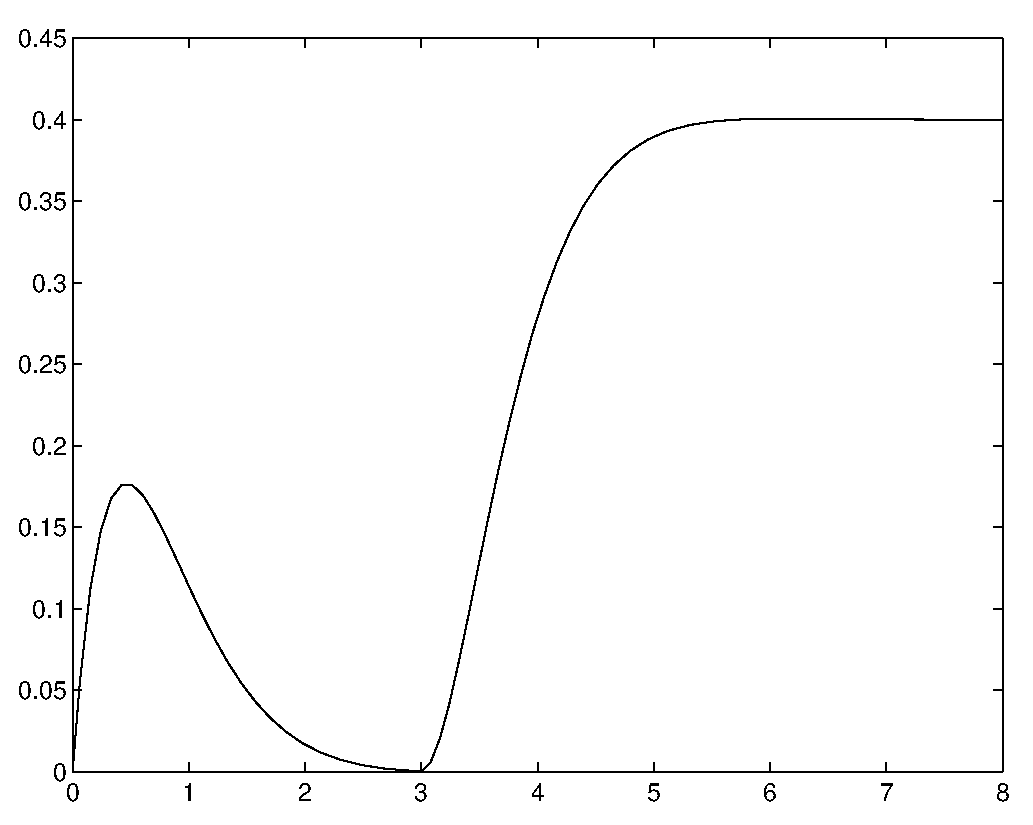
\psfig{file=exfigure/13-4-5a.eps,width=1.8in}
                       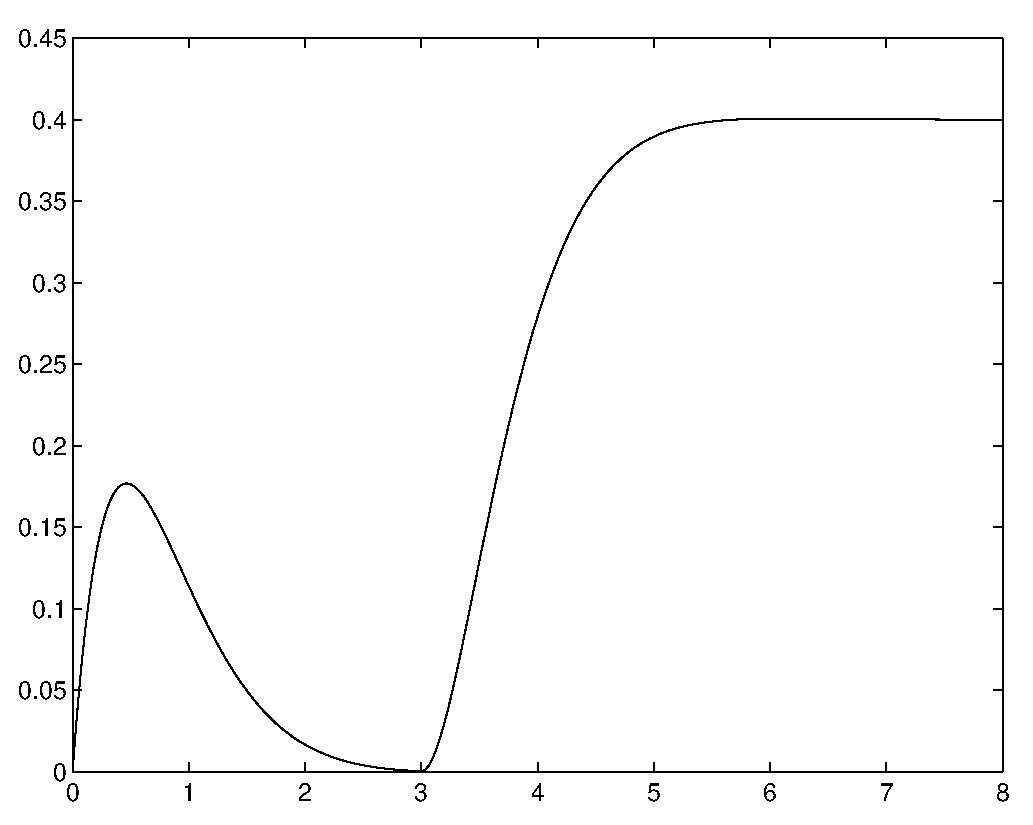
\psfig{file=exfigure/13-4-5b.eps,width=1.8in}
                       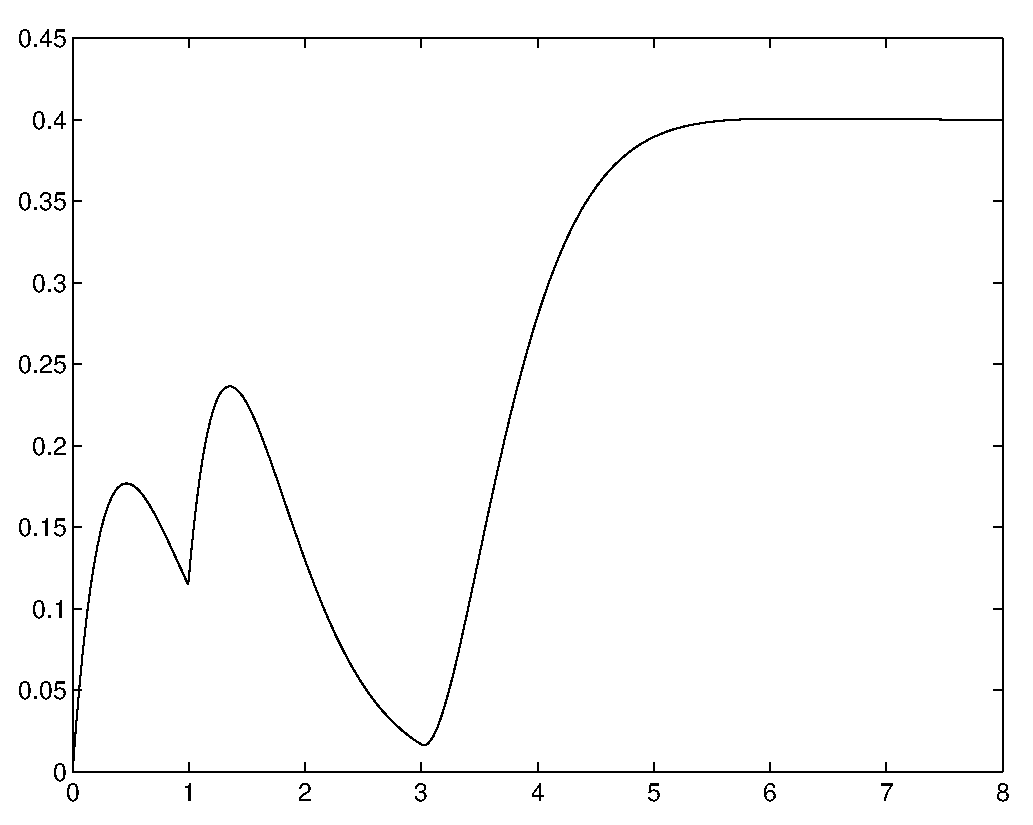
\psfig{file=exfigure/13-4-5c.eps,width=1.8in}}
                \centerline{{\tt eps = 1e-6}\hspace{1.2in}{\tt eps = 1e-8}
\hspace{1.2in}{\tt eps = 1e-10}}
		\exercapthree{c13.4.5}
\end{figure}

